\section{Structure of computations in \dtlifsnn s}
\label{ch:struct}

This section concern itself with the approximation of continuous functions by d.t. LIF-SNN.

In~\cite{nguyen2025timespikeunderstandingrepresentational} the following theorem was proved:
\begin{theorem}\label{thm:approx-snn-constant}
  Let \(f\) be a continuous function on a compact set \(Ω⊂ℝ^{n_0}\). For all \(ε>0\), there exists a d.t. LIF-SNN \(Φ\) with direct encoding, membrane potential output, \(L=2\) and \(T=1\) such that
  \[ \norm{R(Φ)-f}_{∞}≤ε\]
  Moreover, if \(f\) is \(Γ\)-Lipschitz, then \(Φ\) can be chosen with width parameter \(n=(n_1,n_2)\) given by
  \begin{align*}
   n_1 &=\left(\max\left\{\left\lceil \frac{\operatorname{diam}_∞(Ω)}{ε}Γ \right\rceil,1\right\}+1\right)n_0  \\
   n_2 &=\max\left\{\left\lceil \frac{\operatorname{diam}_∞(Ω)}{ε}Γ \right\rceil^{n_0},1\right\}
  \end{align*}
  where \(\operatorname{diam}_∞(Ω)=\sup_{x,y∈Ω}\norm{x-y}_∞\).
\end{theorem}

\begin{proof}
  See~\cite{nguyen2025timespikeunderstandingrepresentational}.
\end{proof}

% TODO: motivation (previous theorem + previous lower bound example), insatisfactory since d.t. SNN. have somewhat linear structure

% TODO: extend to arbitrarily continuous functions by choosing an continuously diff. function close to it
% TODO: extend to continuously differentiable functions apart from lebesgue-zero sets (where they are still continuous?)
% TODO: differentiable, but defined on compact subset of euclidean space???
We will now provide an alternative version of this theorem which uses an increased latency to reduce the number of neurons:
\begin{theorem}\label{thm:approx-snn}
  Let \(f∈𝒞^1(Ω,ℝ^m)\) be a continuously differentiable function on a compact set \(Ω⊂ℝ^n\). For all \(ε>0\), there exists a d.t. LIF-SNN \(Φ\) with direct encoding, membrane potential output, \(L=2\) and
  \begin{align*}
   T &= 2K \\
   n_1 &= n+1 \\ %TODO: add def for K
   n_2 &=K^n·(m+1)
  \end{align*}
  such that
  \[ \norm{R(Φ)-f}_{∞}≤ε\]
\end{theorem}

\begin{lemma}\label{lem:smallest-cube}
  Let \(Ω⊂ℝ^n\) be compact. Then there exists a half-open cube \(C\) with width \(\operatorname{diam}_∞(Ω)\) such that \(Ω⊂\overline{C}\).
\end{lemma}

%TODO: we later use [y,z) instead of [a,b); unify notation
\begin{proof}[\proofofref{lem:smallest-cube}.]
  We can first define \(a≔(\min_{x∈Ω} x_i)_i\) since \(Ω\) is compact We further have \(b≔a+\operatorname{diam}_∞(Ω)·𝟙_n\). We now have \(C≔[a,b)\). Suppose now a point \(y∈Ω∖\overline{C}\) exists. By definition of \(a\), we have \(a≤y\). By definition of \(C\) we further get \(y\nleq b\), and therefore \(∃_ib_i<y_i\) by definition of \(C\). But this means \(\norm{a-y}_∞>\operatorname{diam}_∞(Ω)\).
\end{proof}

% TODO: differentiable, but defined on compact subset of euclidean space???
% TODO: quote formulation?
% TODO: instead of fixing \(ε^{t}\), get supremum of

\newcommand{\dsqe}{δ(ξ)}
\begin{lemma}\label{lem:approx-by-lin}
  Let \(f∈𝒞^1(Ω,ℝ^m)\) be a continuously differentiable function on a compact set \(Ω⊂ℝ^n\) and \(ε>0\). Then there exists a half-open cube \(C\) with \(Ω⊂C\) that can be composed in
  \[ K^n≔\min_{\substack{ξ,θ>0\\ξθ=ε}}\left\{\left\lceil \frac{\operatorname{diam}_∞(Ω)}{\frac{2}{\sqrt{n}}\min(\dsqe ,θ)} \right\rceil\right\}^n \]
  half-open subcubes \((C_i)_{i=1..K^n}\) such that \(Ω⊂C\) and linear functions \(g_i:C_i→ℝ^m\) exists, such that \(\norm{f-g|_Ω}_∞<ε\) for \(g≔\sum_{i=1}^mg_i𝟙_{C_i}\).
  Here \(δ(ε)\) is the modulus of uniform continuity of the total derivative \(dF\).
\end{lemma}

% TODO: fix issue with C_i s not completely fitting in open \sqrt{2}δ(ε) balls due to closed part of C_i
\begin{proof}[\proofofref{lem:approx-by-lin}.]
  By~\autoref{lem:smallest-cube} we have a half-open cube \(C\) with width \(\operatorname{diam}_∞(Ω)\) and \(Ω⊂\overline{C}\).
  Let further \(ε>0\) be given. Since \(Ω\) is compact and \(f∈𝒞^1(Ω,ℝ^m)\), \(dF\) is uniformly continuous on \(Ω\). Let \(δ(ε)\) be \(dF\)s modulus of continuity.
  We will now partition \(C\) in
  \[K^n≔\min_{\substack{ξ,θ>0\\ξθ=ε}}\left\{\left\lceil \frac{\operatorname{diam}_∞(Ω)}{\frac{2}{\sqrt{n}}\min(\dsqe ,θ)} \right\rceil\right\}^n\]
  smaller half-open cubes. There are \(ξ,θ\) such that the minimum in the definition of \(K^n\) is obtained, since we take it over the set of natural numbers.
  The subcubes have width \(w≔\frac{\operatorname{diam}_∞(Ω)}{K}≤\frac{2}{\sqrt{n}}\min(\dsqe,θ)\). % TODO: should be < instead of ≤ in def of w???
  Let us further define \(g_i:C_i→ℝ^m\) by \(g_i(x)≔f(c_i)+df_{c_i}(x-c_i)\) where \(c_i\) is the center of \(C_i\).
  It suffices now to show \(\norm{f|_{C_i}-g_i}_∞<ε\). Let \(x∈C_i\). We get:
  %TODO: ausführlicher

  \begin{align*}
   \norm{f(x)-f(c_i)-df_{c_i}(x-c_i)}_p &= \norm{f(x)-f(c_i)-df_{c_i}(x-c_i)}_p \\
                                    &= \norm{\int_0^1df_{c_i+(x-c_i)t}(x-c_i)dt-df_{c_i}(x-c_i)}_p \\ % h(t)=f(c_i+(x-c_i)t); dh_t = (df_{c_i+(x-c_i)t}∘d_t(t↦c_i+(x-c_i)t))(t) = (df_{c_i+(x-c_i)t}((x-c_i)t))
                                    &≤ \int_0^1\norm{df_{c_i+(x-c_i)t}(x-c_i)-df_{c_i}(x-c_i)}_pdt \\ % Minkowski
                                    &= \int_0^1\norm{(df_{c_i+(x-c_i)t}-df_{c_i})(x-c_i)}_pdt \\
                                    &≤ \int_0^1\norm{(df_{c_i+(x-c_i)t}-df_{c_i})}\norm{x-c_i}_pdt \\
                                    &≤ \int_0^1ξ\norm{x-c_i}_pdt \\ % w≤2\sqrt{n}^{-1}\dsqe %TODO: should be <???
                                    &= ξ\norm{x-c_i}_p \\
                                    &≤ ξθ \\
                                    &= ε
  \end{align*}
\end{proof}

\begin{proof}[\proofofref{thm:approx-snn}.]
  Let a continuously differentiable function \(f∈𝒞^1(Ω,ℝ^m)\) on a compact set \(Ω⊂ℝ^n\) be given. Let there further be a \(ε>0\).
  %TODO: clarify notation [y,z) (line or proper subspace)
  By~\autoref{lem:approx-by-lin} we have a half-open cube \(C=[y,z)\) with \(Ω⊂C\) with composition \(K^n\) half-open subcubes \((C_i)_{i=1..K^n}\) and linear functions \(g_i:C_i→ℝ^m\), such that \(\norm{f-g|_Ω}_∞<ετ\) for a \(g≔\sum_{i=1}^mg_i𝟙_{C_i}\).
  We will now define a \dtlifsnn \(Φ\) with direct input encoding and membrane-potential outputs such that \(\norm{R(Φ)|_Ω-g}_∞<ε(1-τ)\).
  Before anything else we shall set the following basic parameters: \(i^{[l]}(0)=0\), \(α^{[l]}=0\) and \(β^{[l]}=ϑ^{[l]}=1\).
  We obtain the simplified equations:
  \begin{align*}
    p^{[l]}(t) & = u^{[l]}(t-1)+W^{[l]}s^{[l-1]}(t)+V^{[l]}s^{[l]}(t-1)+b^{[l]} \\
    s^{[l]}(t) & = H(p^{[l]}(t)-1_{n_l}) \\
    u^{[l]}(t) & = p^{[l]}(t)-s^{[l]}(t)
  \end{align*}
  % TODO: graphic
  The intuitive idea is the following… %TODO
  We define the \(i\)-th neuron of the first \(n\) of the first layer by parameters \(w=\frac{1}{z_i-y_i}e_i\), \(b=-\frac{y_i}{z_i-y_i}\), \(v=-e_{n+1}\), \(u_0=0\), \(i_0=0\).
  We obtain
  \[ p^{[1]}_i(t) = u^{[1]}_i(t-1)+\frac{1}{z_i-y_i}s_i^{[0]}(t)-s^{[1]}_{n+1}(t-1)-\frac{y_i}{z_i-y_i} \]
  and therefore \(1=s^{[1]}_i(t)⇔\)

  % TODO: why K≠0
  % TODO: check on „off by one errors“
  We further define the \(n+1\)-th neuron by parameters \(w=0\), \(b=1\), \(v=e_{n+1}\), \(u_0=-(K-1)\), \(i_0=0\).

  Let us now regard the second layer.
\end{proof}

%TODO: remark about SNN construction. By adding more neurons to first layer ((K-1)n to be exact) you can half the required time steps.

%TODO: mollification


comparison:
sin mit kleiner ampitude, extrem hoher frequenz

%TODO: better for ε→0
\begin{theorem}

\end{theorem}

The proof works by first showing that a continuous function can be arbitrarily approximated by step functions, in particular by step functions constant on hypercubes in \(Ω\).
Then the d.t. LIF-SNN is constructed by using the first layer to cut the input space by hyperplanes along the cubes and using the second layer to represent the hypercubes.

\autoref{fig:sinus} shows a sinus function getting approximated in this way.

\begin{figure}[h!]
  \centering
  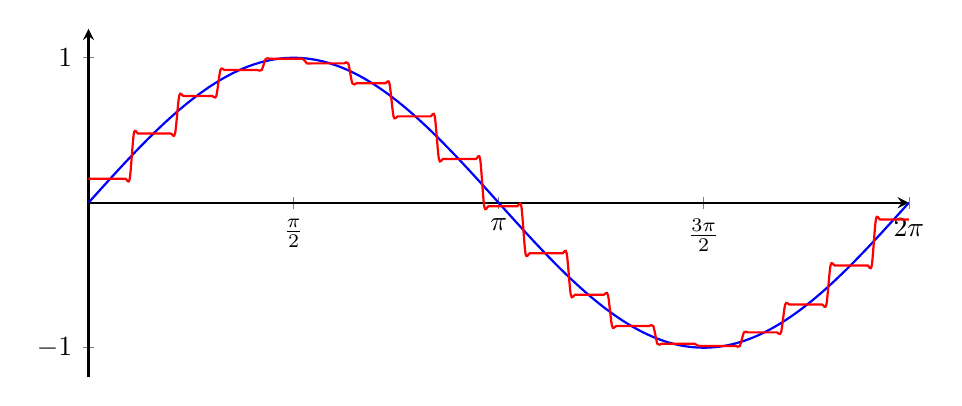
\begin{tikzpicture}
    \begin{axis}[
      axis lines=middle,
      xmin=0, xmax=2*pi,
      ymin=-1.2, ymax=1.2,
      xtick={0, pi/2, pi, 3*pi/2, 2*pi},
      xticklabels={$0$, $\frac{\pi}{2}$, $\pi$, $\frac{3\pi}{2}$, $2\pi$},
      ytick={-1, 0, 1},
      domain=0:2*pi,
      samples=200,
      smooth,
      thick,
      legend style={at={(0.5,-0.2)}, anchor=north},
      width=12cm,
      height=6cm
      ]
      \addplot[blue]{sin(deg(x))};
      \addplot[red]{(-cos(deg(floor(x*3+1)/3))+cos(deg(floor(x*3)/3)))*3};
    \end{axis}
  \end{tikzpicture}
  \caption{A \dtlifsnn approximating a sinus wave}
  \label{fig:sinus}
\end{figure}


% TODO: encoding with fewer layers for on finite segments continuously differentiable functions
